\section{Methodology}
\label{sec:methodology}

Building on our observation that efficiency claims require mechanism-level validation, we design both a temporal dynamic attention architecture and a verification framework for testing whether proposed mechanisms actually operate.

\subsection{Overview}

Our approach has two components:

\begin{enumerate}
    \item \textbf{Temporal Dynamic Attention:} An attention mechanism where weights evolve across $T$ internal steps within each layer, with K and V projections computed once and Q reprojected at each step.

    \item \textbf{Sub-Hypothesis Verification:} A framework decomposing the efficiency claim into four testable sub-hypotheses with explicit gates and falsification criteria.
\end{enumerate}

\subsection{Temporal Dynamic Attention Architecture}

\subsubsection{Design Rationale}

Standard attention computes Q, K, V projections once per layer, applies softmax, and outputs. We hypothesize that allowing attention weights to \emph{evolve} across internal time steps could reduce redundant computation---if temporal refinement converges toward task-relevant patterns, fewer full recomputations may be needed.

\textbf{Core architecture:}
\begin{align}
\text{Input:} \quad & X \in \mathbb{R}^{\text{seq\_len} \times d_{\text{model}}} \nonumber \\
Q_1 = X \cdot W_Q, \quad & K = X \cdot W_K, \quad V = X \cdot W_V \nonumber \\
\text{For } t = 1 \text{ to } T: \quad & A_t = \text{softmax}\left(\frac{Q_t \cdot K^T}{\sqrt{d_k}}\right) \nonumber \\
& Q_{t+1} = \text{gate}(Q_t, A_t \cdot V \cdot W_Q') \nonumber \\
\text{Output} = & \, A_T \cdot V \cdot W_O \nonumber
\end{align}

\textbf{Key design decisions:}

\begin{enumerate}
    \item \textbf{K/V reuse:} K and V are computed once and reused across temporal steps. This amortizes projection cost.
    \begin{itemize}
        \item \emph{Rationale:} K/V capture input content; only Q (the query) needs refinement.
    \end{itemize}

    \item \textbf{Learned gating:} A gating mechanism controls how much each temporal step modifies Q.
    \begin{itemize}
        \item \emph{Rationale:} Prevents unbounded divergence; allows learning when refinement helps.
    \end{itemize}

    \item \textbf{Configurable $T$:} The number of temporal steps is a hyperparameter ($T \in \{1, 2, 3, \ldots\}$).
    \begin{itemize}
        \item \emph{Rationale:} Enables testing the efficiency-vs-quality tradeoff at different iteration counts.
    \end{itemize}
\end{enumerate}

\subsubsection{Computational Cost Analysis}

\begin{align}
\text{Standard Attention:} \quad & \text{FLOPs} = Q_{\text{proj}} + K_{\text{proj}} + V_{\text{proj}} + \text{Attention} + O_{\text{proj}} \nonumber \\
\text{Temporal ($T$ steps):} \quad & \text{FLOPs} = Q_{\text{proj}} + K_{\text{proj}} + V_{\text{proj}} + T \times (Q_{\text{reproj}} + \text{Attention}) + O_{\text{proj}} \nonumber
\end{align}

Reducing $T$ from 3 to 2 removes 1/3 of the iterative overhead. Since Q reprojection ($W_Q'$) is cheaper than full Q/K/V projection, overhead per step is bounded.

\subsection{Sub-Hypothesis Verification Framework}

Rather than evaluating only end-to-end efficiency, we decompose our claim into four sub-hypotheses:

\subsubsection{H-E1: Existence (MUST\_WORK Gate)}

\textbf{Statement:} Temporal dynamic attention can be implemented and trains stably.

\textbf{Success criteria:} Model perplexity within 10\% of baseline, no gradient explosion.

\textbf{If FAIL:} Core mechanism infeasible; STOP pipeline.

\subsubsection{H-M1: Mechanism -- Efficiency (MUST\_WORK Gate)}

\textbf{Statement:} Reducing temporal steps decreases FLOPs while maintaining perplexity.

\textbf{Success criteria:} FLOP reduction $\geq$ 10\%, perplexity within $\pm$5\% of T=3 baseline.

\textbf{If FAIL:} Efficiency claim not validated.

\subsubsection{H-M2: Mechanism -- Convergence (SHOULD\_WORK Gate)}

\textbf{Statement:} Attention patterns converge (entropy decreases) across temporal steps.

\textbf{Success criteria:} Entropy reduction $>$ 5\% from step 1 to final step.

\textbf{If FAIL:} Convergence hypothesis falsified, but efficiency may still hold through other mechanisms.

\subsubsection{H-C1: Condition -- Scaling (SHOULD\_WORK Gate)}

\textbf{Statement:} Efficiency gains scale with sequence length.

\textbf{Success criteria:} Positive scaling coefficient.

\textbf{If FAIL:} Efficiency is constant, not scaling.

\subsubsection{Gate Hierarchy}

\begin{verbatim}
MUST_WORK gates (H-E1, H-M1):
  Failure -> Pipeline stops, core claim invalid

SHOULD_WORK gates (H-M2, H-C1):
  Failure -> Continue with limitation noted
\end{verbatim}

This hierarchy allows distinguishing between \emph{core} efficiency results and \emph{proposed} mechanistic explanations.

\subsection{Implementation}

We implement temporal dynamic attention in PyTorch, modifying the standard multi-head attention module. Training uses standard language modeling on WikiText-103 with AdamW optimizer. FLOP profiling uses the \texttt{thop} library. Attention entropy computed as $H = -\sum p \log p$ over attention distributions.

\begin{figure}[t]
    \centering
    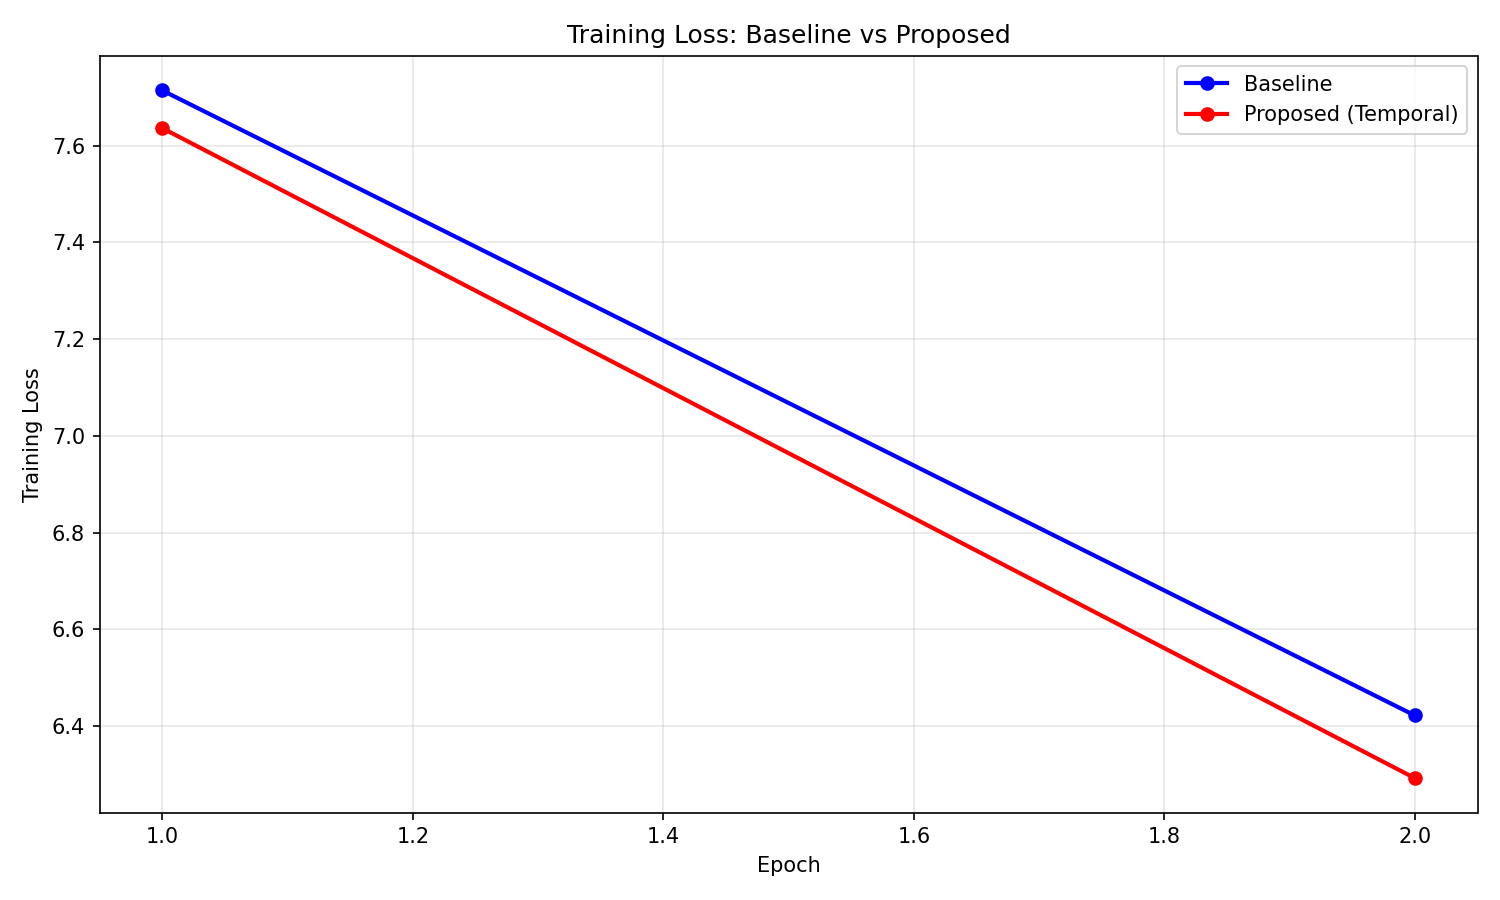
\includegraphics[width=0.9\columnwidth]{figures/loss_curves.png}
    \caption{Training loss curves demonstrating stable convergence of the temporal attention mechanism.}
    \label{fig:loss_curves}
\end{figure}
